\documentclass[a4paper, 12pt]{report}
\usepackage{cmap}
\usepackage{amssymb}
\usepackage{amsmath}
\usepackage{graphicx}
\usepackage{amsthm}
\usepackage{upgreek}
\usepackage{setspace}
\setcounter{secnumdepth}{5}
\setcounter{tocdepth}{5}
\usepackage[T2A]{fontenc}
\usepackage[utf8]{inputenc}
\usepackage[normalem]{ulem}
\usepackage{mathtext} % русские буквы в формулах
\usepackage[left=2cm,right=2cm, top=2cm,bottom=2cm,bindingoffset=0cm]{geometry}
\usepackage[english,russian]{babel}
\usepackage[unicode]{hyperref}
\newenvironment{Proof} % имя окружения
{\par\noindent{$\blacklozenge$}} % команды для \begin
{\hfill$\scriptstyle\boxtimes$}
\newcommand{\Rm}{\mathbb{R}}
\newcommand{\Cm}{\mathbb{C}}
\newcommand{\Z}{\mathbb{Z}}
\newcommand{\I}{\mathbb{I}}
\newcommand{\N}{\mathbb{N}}
\newcommand{\rank}{\operatorname{rank}}
\newcommand{\Ra}{\Rightarrow}
\newcommand{\ra}{\rightarrow}
\newcommand{\FI}{\Phi}
\newcommand{\Sp}{\text{Sp}}
\renewcommand{\leq}{\leqslant}
\renewcommand{\geq}{\geqslant}
\renewcommand{\alpha}{\upalpha}
\renewcommand{\beta}{\upbeta}
\renewcommand{\gamma}{\upgamma}
\renewcommand{\delta}{\updelta}
\renewcommand{\varphi}{\upvarphi}
\renewcommand{\phi}{\upvarphi}
\renewcommand{\tau}{\uptau}
\renewcommand{\lambda}{\uplambda}
\renewcommand{\psi}{\uppsi}
\renewcommand{\mu}{\upmu}
\renewcommand{\omega}{\upomega}
\renewcommand{\d}{\partial}
\renewcommand{\xi}{\upxi}
\renewcommand{\epsilon}{\upvarepsilon}
\newcommand{\intx}{\int\limits_{x_0}^x}
\newcommand\Norm[1]{\left\| #1 \right\|}
\newcommand{\sumk}{\sum\limits_{k=0}^\infty}
\newcommand{\sumi}{\sum\limits_{i=0}^\infty}
\newtheorem*{theorem}{Теорема}
\newtheorem*{cor}{Следствие}
\newtheorem*{lem}{Лемма}
\begin{document}
	\section*{Постановка задачи.}
	\begin{enumerate}
		\item Построить сетевой график для максимальной ($t_\text{пес}$) продолжительности всех его работ, рассчитать наиболее ранние и наиболее поздние сроки наступления событий, найти критический путь, определить полные и независимые резервы времени всех работ и коэффициенты напряженности некритических дуг.
		\item Для трехпараметрической модели найти ожидаемое время выполнения проекта, определить вероятность выполнения проекта не позднее заданного срока, найти интервал гарантированного (с вероятностью $Р = 0,9973$) времени выполнения проекта, оценить максимально возможный срок выполнения проекта с заданной надежностью.\\
		Выполнить те же расчеты для двухпараметрической модели. Сравнить результаты.
		\item Считая $t_\text{пес}$ продолжительностью работы с минимальной допустимой интенсивностью ($t_\text{пес} = t_\text{max}$), а $t_\text{опт}$ – продолжительностью работы с максимальной возможной интенсивностью ($t_\text{опт} = t_\text{min}$), найти оптимальный по стоимости вариант выполнения проекта.\\
		Минимизировать стоимость проекта при минимально возможном сроке его исполнения.
	\end{enumerate}
\begin{center}
	\includegraphics[scale=0.5]{"img1"}
\end{center}
	Директивный (заданный) срок выполнения проекта $T_\text{дир} = 30 \ \text{дней}$.\\
	Заданная надежность $\gamma = 0,95$.\\
	Стоимость одного дня проекта равна $12$ денежным единицам: $S = 12$.
	\section*{Решение задачи}
	\subsection*{Пункт 1}
	Сначала строим структурный сетевой график и вводим правильную нумерацию событий:
$$
	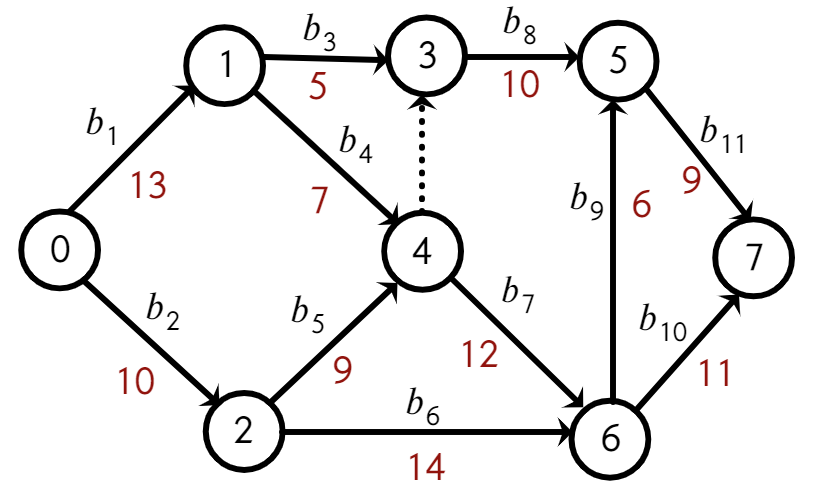
\includegraphics[scale=0.5]{img2}
$$
	Наиболее ранние сроки наступления событий находим по формуле:
	$$T_p(i)=\max\limits_{j\subset i}\{T_p(j)+t_{ji}\},$$
	где максимум берется по всем событиям $j$, непосредственно предшествующим событию $i$. Начальному событию присваиваем $T_p(0)=0$.
	Тогда:$$\begin{cases}
	T_p(1)=T_p(0)+t_{01}=0+13=13;\\
	T_p(2)=T_p(0)+t_{02}=0+10=10;\\
	T_p(3)=\max\{T_p(1)+t_{13}, T_p(4)+t{34}\}\max\{13+5, 20+0\}=20;\\
	T_p(4)=\max\{T_p(2)+t_{24},T_p(1)+t_{14}\}=\max\{10+9, 13+7\}=20;\\
	T_p(5)=\max\{T_p(3)+t_{35},T_p(6)+t_{56}\}=\{20+10, 32+6\}=38;\\
	T_p(6)=\max\{T_p(4)+t_{46},T_p(2)+t_{26}\}=\max\{20+12, 10+14\}=32;\\
	T_p(7)=\max\{T_p(5)+t_{57},T_p(6)+t_{67}\}=\max\{38+9, 32+11\}=47.
	\end{cases}
	$$
	Итак, критическое время $T_\text{кр}$ = 47. Минимальный срок выполнения
	проекта -- 47 дней.\\
	Наиболее поздние сроки наступления событий находим по формуле:
	$$T_\text{п}(i)=\min\limits_{j\supset i}\{T_\text{п}(j)-t_{ij}\},$$
	где минимум берется по всем событиям $j$, непосредственно следующим за событием $i$. Конечному событию присваиваем наиболее поздний срок наступления, равный критическому времени: $T_\text{п}(7)=T_\text{кр}=47$.
	Тогда:
	$$
	\begin{cases}
	T_\text{п}(6)=T_\text{п}(6)-t_{67}=-0=35;\\
	T_\text{п}(5)=T_\text{п}(7)-t_{57}=47-9=38;\\
	T_\text{п}(4)=\min\{T_\text{п}(5)-t_{45},T_\text{п}(6)-t_{46},T_\text{п}(7)-t_{47}\}=\min\{35-9, 35-8, 44-11\}=26;\\
	T_\text{п}(3)=\min\{T_\text{п}(4)-t_{34}, T_\text{п}(6)-t_{36}\}=\min\{26-6, 35-10\}=20;\\
	T_\text{п}(2)=\min\{T_\text{п}(3)-t_{23}, T_\text{п}(4)-t_{24}, T_\text{п}(7)-t_{27}\}=\min\{20-6, 44-10\}=14;\\
	T_\text{п}(1)=T_\text{п}(3)-t_{13}=20-5=15;\\
	T_\text{п}(0)=\min\{T_\text{п}(1)-t_{01},T_\text{п}(2)-t_{02}\}=\min\{15-15, 14-7\}=0.
	\end{cases}
	$$
	Результаты расчетов отразим на сетевом графике. Ранние сроки
	наступления событий запишем над кружками, изображающими эти
	события, поздние сроки наступления событий -- под кружками.
	%	$$\includegraphics[width=15cm]{img/5.3.JPG}$$
	Критическое время $T_\text{кр}$ = 44.\\
	Временные характеристики событий представлены в таблице: \\
	\begin{tabular}{ |p{3cm}||p{3cm}||p{3cm}||p{3cm}|  }
		\hline
		Событие & Ранний срок $T_p(i)$ & Поздний срок $T_\text{п}(i)$ & Резерв времени $R(i)$\\
		\hline
		* 0 & 0 & 0 & 0\\
		* 1 & 15 & 15 & 0\\
		\;\;\;2 & 7 & 14 & 7\\
		* 3 & 20 & 20 & 0\\
		* 4 & 26 & 26 & 0\\
		* 5 & 35 & 35 & 0\\
		* 6 & 35 & 35 & 0\\
		* 7 & 44 & 44 & 0\\
		\hline
	\end{tabular}\\\\
	Резервы времени событий найдены по формуле $R(i)=T_\text{п}(i)-T_p(i)$.\\
	Критический путь проходит через события с нулевым резервом
	времени, т. е. через события $0$, $1$, $3$, $4$, $5$, $6$, $7$.\\
	Найдем резервы времени работ.\\
	Наиболее ранний возможный срок начала работы $b_k = (i, j)$ равен
	наиболее раннему сроку наступления события $i$: $S_p(b_k) = T_p(i)$, а наиболее поздний допустимый срок окончания работы $b_k = (i, j)$ равен
	наиболее позднему сроку наступления события $j$: $E_\text{п}(b_k) = T_\text{п}(j)$.\\
	Полный резерв времени работ найдем по формуле:
	$$r_\text{п}(b_k)=r_\text{п}(i,j)=T_\text{п}(j)-T_p(i)-t_{ij}=E_\text{п}(b_k)-S_p(b_k)-t_{ij}.$$
	Независимый резерв времени работ найдем по формуле:
	$$r_\text{н}(b_k)=r_\text{н}(i,j)=T_p(j)-T_\text{п}(i)-t_{ij}.$$
	Сведем полученные данные в таблицу:\\
	\begin{tabular}{ |p{2.5cm}||p{5cm}||p{1cm}||p{1cm}||p{1cm}||p{1cm}|  }
		\hline
		Работа $b_k=(i,j)$& Продолжительность работы, $t(b_k)=t_{ij}$ & $S_p(b_k)$ & $E_\text{п}(b_k)$ & $r_\text{п}(b_k)$ & $r_\text{н}(b_k)$\\
		\hline
		* $b_1=(0,1)$ & 15 & 0 & 15 & 0 & 0\\
		\;\;\;$b_2=(0,2)$ & 7 & 0 & 14 & 7 & 0\\
		* $b_3=(1,3)$ & 5 & 15 & 20 & 0 & 0\\
		\;\;\;$b_4=(2,3)$ & 6 & 6 & 20 & 8 & 0\\
		\;\;\;$b_5=(2,4)$ & 8 & 7 & 26 & 11 & 4\\
		* $b_6=(3,4)$ & 6 & 20 & 26 & 0 & 0\\
		\;\;\;$b_7=(3,6)$ & 10 & 20 & 35 & 5 & 5\\
		\;\;\;$b_8=(4,6)$ & 8 & 26 & 35 & 1 & 1\\
		* $b_9=(4,5)$ & 9 & 26 & 35 & 0 & 0\\
		\;\;\;$b_{10}=(4,7)$ & 11 & 26 & 44 & 7 & 7\\
		\;\;\;$b_{11}=(2,7)$ & 10 & 7 & 44 & 27 & 20\\
		* $b_{12}=(6,7)$ & 9 & 35 & 44 & 0 & 0\\
		* $\varphi=(5,6)$ & 0 & 35 & 35 & 0 & 0\\
		\hline
	\end{tabular}\\\\
	Работа $\varphi = (5, 6)$ -- фиктивная работа.\\
	Критические работы -- $b_1$, $b_3$, $b_6$, $b_9$, $b_{12}$, $\varphi$. Резервы времени этих работ равны нулю. Выделим критический путь жирными красными стрелками (фиктивная работа - розовая).
	%$$\includegraphics[width=15cm]{img/5.4.JPG}$$
	Резерв времени некритической дуги $b$ находим как разность между
	длиной замыкающего критического участка и длиной самой некритической дуги:
	$$R(b)-a-b.$$
	Коэффициент напряжённости некритической дуги определим по формуле:
	$$N(b)=\frac{b}{a}=1-\frac{R(b)}{a}.$$
	Резервы времени и коэффициенты напряженности некритических
	дуг представим в таблице: \\
	\begin{tabular}{ |p{3cm}||p{1cm}||p{1cm}||p{4cm}||p{4cm}|}
		\hline
		Некритические дуги& $a$ & $b$ & Резерв времени дуги, $R(b)$ & Коэффициент напряжённости дуги, $N(b)$\\
		\hline
		$(0,2,3)$ & 20 & 13 & 7 & $\frac{13}{20}=0,650$\\
		$(0,2,4)$&26&15&11&$\frac{15}{26}\approx0,577$\\
		$(0,2,7)$&44&17&27&$\frac{17}{44}\approx0,386$\\
		$(0,2,4,7)$&44&26&18&$\frac{26}{44}\approx0,591$\\
		$(0,2,3,6)$&35&23&12&$\frac{23}{35}\approx0,657$\\
		$(0,2,4,6)$&35&23&12&$\frac{13}{20}\approx0,657$\\
		$(4,6)$&9&8&1&$\frac{8}{9}\approx0,889$\\
		$(3,6)$&15&10&5&$\frac{10}{15}\approx0,667$\\
		$(4,7)$&18&11&7&$\frac{11}{18}=0,611$\\
		\hline
	\end{tabular}\\\\
	Дуги, коэффициент напряженности которых $N(b) > 0,8$, составляют критическую зону, дуги с коэффициентом напряженности
	$0,6 \leq N(b) \leq 0,8$ образуют подкритическую зону, а дуги с коэффициентом $N(b) < 0,6$ дают резервную зону. В нашем случае в критическую зону попадает критический путь и дуга $(4,6)$, в подкритической зоне
	находится дуги $(0,2,3)$, $(0,2,3,6)$, $(0,2,4,6)$, $(3,6)$, $(4,7)$. Она быстрее
	всего может перейти на критический путь. Дуги $(0,2,4)$, $(0,2,7)$, $(0,2,4,7)$ образуют резервную зону.\\\\
	\textbf{\textit{Пункт 2.}}\\\\
	Найдем ожидаемую продолжительность работ $(t_\text{ож})$ для трехпараметрической модели по формуле:
	$$t_\text{ож}=\frac{t_\text{пес}+4t_\text{вер}+t_\text{опт}}{6}.$$
	Для упрощения дальнейших вычислений округляем полученные
	величины до целых чисел (по правилам округления с избытком и недостатком).\\
	Для сравнения найдем также ожидаемую продолжительность работ $(t_\text{
		ож}^*)$ для двухпараметрической модели по формуле:
	$$t_\text{ож}^*=\frac{3t_\text{пес}+2t_\text{опт}}{5}.$$
	Двухпараметрическая модель проще, но дает менее точные оценки.\\
	Для вычисления дисперсий продолжительностей работ воспользуемся формулой:
	$$\sigma^2(t_\text{ож})=\left(\frac{t_\text{пес}-t_\text{опт}}{6}\right)^2.$$
	Дополним исходную таблицу полученными значениями:\\
	\begin{tabular}{ |p{3cm}||p{4cm}||p{1cm}||p{1cm}||p{1cm}||p{1cm}||p{1cm}||p{1cm}|}
		\hline
		Работа & Опирается на работы & $t_\text{пес}$ & $t_\text{вер}$ & $t_\text{опт}$ & $t_\text{ож}$ & $t_\text{ож}^*$ & $\sigma^2$\\
		\hline
		$b_1$ & -- & 15 & 9 & 3 & 9 & 10 & 4,00\\
		$b_2$ & -- & 7 & 5 & 4 & 5 & 6 & 0,25\\
		$b_3$ & $b_1$ & 5 & 3 & 2 & 3 & 4 & 0,25\\
		$b_4$ & $b_2$ & 6 & 4 & 1 & 4 & 4 & 0,69\\
		$b_5$ & $b_2$ & 8 & 6 & 2 & 6 & 6 & 1,00\\
		$b_6$ & $b_3,b_4$ & 6 & 4 & 2 & 4 & 4 & 0,44\\
		$b_7$ & $b_3,b_4$ & 10 & 5 & 3 & 6 & 7 & 1,36\\
		$b_8$ & $b_5,b_6$ & 8 & 5 & 1 & 5 & 5 & 1,36\\
		$b_9$ & $b_5,b_6$ & 9 & 7 & 4 & 7 & 7 & 0,69\\
		$b_{10}$ & $b_5,b_6$ & 11 & 8 & 6 & 8 & 9 & 0,69\\
		$b_{11}$ & $b_2$ & 10 & 12 & 3 & 10 & 7 & 1,36\\
		$b_{12}$ & $b_7,b_8,b_9$ & 9 & 5 & 2 & 5 & 6 & 1,36\\
		\hline
	\end{tabular}\\\\
	Таким образом трехпараметрическая модель сведена к однопараметрической.\\
	Теперь можно построить сетевой график и рассчитать его временные характеристики.
	%$$\includegraphics[width=15cm]{img/5.5.JPG}$$
	\begin{tabular}{ |p{3cm}||p{4cm}||p{1cm}||p{1cm}|}
		\hline
		Работа & Опирается на работы & $t_\text{ож}$ & $\sigma^2$\\
		\hline
		* $b_1$ & -- & 9 & 4,00\\
		\;\;\;$b_2$ & --  & 5 &  0,25\\
		* $b_3$ & $b_1$ & 3 & 0,25\\
		\;\;\;$b_4$ & $b_2$ & 4 & 0,69\\
		\;\;\;$b_5$ & $b_2$ & 6 & 1,00\\
		* $b_6$ & $b_3,b_4$& 4  & 0,44\\
		\;\;\;$b_7$ & $b_3,b_4$ & 6 & 1,36\\
		\;\;\;$b_8$ & $b_5,b_6$ & 5 & 1,36\\
		* $b_9$ & $b_5,b_6$  & 7 & 0,69\\
		\;\;\;$b_{10}$ & $b_5,b_6$  & 8 & 0,69\\
		\;\;\;$b_{11}$ & $b_2$ & 10 &  1,36\\
		* $b_{12}$ & $b_7,b_8,b_9$ & 5 & 1,36\\
		\hline
	\end{tabular}\\\\
	Ожидаемое критическое время $T_\text{кр}$ = 28.\\
	На критическом пути лежат работы $b_1$, $b_3$, $b_6$, $b_9$, $b_{12}$, $\varphi$ (фиктивная работа).\\
	Найдем дисперсию критического пути.
	$$\sigma^2_\text{кр}=\sigma^2(b_1)+\sigma^2(b_3)+\sigma^2(b_6)+\sigma^2(b_9)+\sigma^2(b_{12})=4,00+0,25+0,44+0,69+1,36=6,74.$$
	Среднеквадратическое отклонение критического пути:
	$$\sigma_\text{кр}=\sqrt{6,74}\approx 2,60.$$
	Найдем вероятность того, что проект будет выполнен не позднее
	заданного срока ($T_\text{дир}$ = $29$ дней):
	$$P(t_\text{кр}\leq 29)=0,5+\Phi\left(\frac{29-28}{2,60}\right)=0,5+\Phi(0,38)=0,5+0,1480\approx 0,65.$$
	Таким образом, имеются шансы в $65\%$ выполнить проект в заданный срок.\\
	Найдем интервал гарантированного времени выполнения проекта.\\
	Воспользуемся правилом «трех сигм»: $3\sigma_\text{кр} = 3\cdot 2,60=7,80\approx 8$, т.е с вероятностью почти $0,9973$ проект будет выполнен за $28\pm 8$ дней.
	$$P(20\leq t_\text{кр}\leq 36)=P(|t_\text{кр}-28|\leq 8)\approx P(|t_\text{кр}-28|\leq 3\sigma_\text{кр})=0,9973.$$
	(Расчет значения:
	$$P(20\leq t_\text{кр}\leq 36)=P(|t_\text{кр}-28|\leq 8)=2\Phi(\frac{8}{2,60})=2\Phi(3,08)=2\cdot0,49865=0,9973)$$ 
	$$P(t_\text{кр}\leq 36)=0,5+\Phi\left(\frac{36-28}{2,60}\right)=0,5+\Phi(3,08) = 0,99865$$
	Следовательно, можно с большой долей уверенности гарантировать, что максимальный срок выполнения проекта не превысит $36$ дней.\\
	Оценим максимально возможный срок $T$ выполнения проекта с заданной надежностью $\gamma = 0,90$.\\
	По таблице значений функции Лапласа найдем доверительный коэффициент $z_\gamma$ для заданной надежности $\gamma$.\\
	Так как $P(|t_\text{кр}-T_\text{кр}|\leq z_{0,90}\sigma_\text{кр})=2\Phi\left(\frac{z_{0,90}\sigma_\text{кр}}{\sigma_\text{кр}}\right)=2\Phi(z_{0,90})=0,90$, то из $2\Phi(z_\text{0,90})=0,90\Longrightarrow \Phi(z_{0,90})=0,45\Longrightarrow z_{0,90}=1,65$ и $P(|t_\text{кр}-28|\leq 1,65\cdot 2,60)=P(|t_\text{кр}-28|\leq 4,29)=P(23,71\leq t_\text{кр}\leq 32,29)=0,90$.\\
	Это значит, что с надежностью $0,90$ проект будет завершен в период от 23 до 33 дней.\\
	Здесь использована функция Лапласа вида $\Phi(x)=\frac{1}{\sqrt{2\pi}}\int\limits_0^xe^{\frac{-t^2}{2}}dt$.\\
	Необходимо помнить, что использовалось, что функция Лапласа данного вида нечетная, т.е. $\Phi(-x)=-\Phi(x)$, а при $x\geq 5$ значение $\Phi(x)\approx 0,5$.\\\\
	Рассмотрим теперь двухпараметрическую модель. Такая модель
	используется в тех случаях, когда сложно определить наиболее вероятные продолжительности выполнения отдельных работ. Ожидаемая
	продолжительность работ ($t_\text{ож}^*$) для двухпараметрической модели
	нами уже вычислена. Среднеквадратическое отклонение этих продолжительностей то же, что и у трехпараметрической модели.\\
	Итак, для двухпараметрической модели имеются следующие данные, представленные в таблице:\\
	\begin{tabular}{ |p{3cm}||p{4cm}||p{1cm}||p{1cm}||p{1cm}||p{1cm}||p{1cm}||p{1cm}|}
		\hline
		Работа & Опирается на работы & $t_\text{пес}$ & $t_\text{опт}$& $t_\text{ож}^*$ & $\sigma^2$\\
		\hline
		$b_1$ & -- & 15 & 3 & 10 & 4,00\\
		$b_2$ & -- & 7  & 4 & 6 & 0,25\\
		$b_3$ & $b_1$ & 5 & 2  & 4 & 0,25\\
		$b_4$ & $b_2$ & 6  & 1  & 4 & 0,69\\
		$b_5$ & $b_2$ & 8 & 2  & 6 & 1,00\\
		$b_6$ & $b_3,b_4$ & 6  & 2  & 4 & 0,44\\
		$b_7$ & $b_3,b_4$ & 10  & 3  & 7 & 1,36\\
		$b_8$ & $b_5,b_6$ & 8  & 1  & 5 & 1,36\\
		$b_9$ & $b_5,b_6$ & 9  & 4  & 7 & 0,69\\
		$b_{10}$ & $b_5,b_6$ & 11 & 6  & 9 & 0,69\\
		$b_{11}$ & $b_2$ & 10  & 3  & 7 & 1,36\\
		$b_{12}$ & $b_7,b_8,b_9$ & 9 & 2 & 6 & 1,36\\
		\hline
	\end{tabular}\\\\
	Проведем анализ полученной модели. Найдем временные характеристики событий и работ. Построим структурный сетевой график.
	%$$\includegraphics[width=15cm]{img/5.6.JPG}$$
	Сроки наступления и резервы времени событий указаны в таблице: \\
	\begin{tabular}{ |p{3cm}||p{3cm}||p{3cm}||p{3cm}|  }
		\hline
		Событие & Ранний срок $T_p(i)$ & Поздний срок $T_\text{п}(i)$ & Резерв времени $R(i)$\\
		\hline
		* 0 & 0 & 0 & 0\\
		* 1 & 10 & 10 & 0\\
		\;\;\;2 & 6 & 10 & 4\\
		* 3 & 14 & 14 & 0\\
		* 4 & 18 & 18 & 0\\
		* 5 & 25 & 25 & 0\\
		* 6 & 25 & 25 & 0\\
		* 7 & 31 & 31 & 0\\
		\hline
	\end{tabular}\\\\
	Критический путь проходит через события с нулевым резервом
	времени, т. е. через события $0$, $1$, $3$, $4$, $5$, $6$, $7$. Критическое время $T_\text{кр}$ = 31
	день.\\
	Характеристики работ указаны в таблице: \\
	\begin{tabular}{ |p{4cm}||p{1cm}||p{1cm}||p{1cm}||p{1cm}||p{1cm}||p{1cm}||p{1cm}||p{1cm}|  }
		\hline
		Работа $b_k=(i,j)$& $t_\text{ож}^*$& $\sigma^2$ & $S_p(b_k)$ & $S_\text{п}(b_k)$ & $E_p(b_k)$ & $E_\text{п}(b_k)$ & $r_\text{п}(b_k)$ & $r_\text{н}(b_k)$\\
		\hline
		* $b_1=(0,1)$ & 10 & 4,00 & 0 & 0 & 10 & 10 &0&0\\
		\;\;\;$b_2=(0,2)$ & 6 & 0,25 & 0 & 4 & 6 & 10 &4&0\\
		* $b_3=(1,3)$ & 4 & 0,25 & 10 & 10 & 14 & 14&0&0 \\
		\;\;\;$b_4=(2,3)$ & 4 & 0,69 & 6 & 10 & 10 & 14 &4&0\\
		\;\;\;$b_5=(2,4)$ & 6 & 1,00 & 6 & 12 & 12 & 18 &6&2\\
		* $b_6=(3,4)$ & 4 & 0,44 & 14 & 14 & 18 & 18 &0&0\\
		\;\;\;$b_7=(3,6)$ & 7 & 1,36 & 14 &  18 & 21 & 25 &4&4\\
		\;\;\;$b_8=(4,6)$ & 5 & 1,36 & 18 & 20 & 23 &25&2&2\\
		* $b_9=(4,5)$ & 7 & 0,69 & 18 & 18 & 25 &25&0&0\\
		\;\;\;$b_{10}=(4,7)$ & 9 & 0,69 & 18 & 22 & 27 &31&4&4\\
		\;\;\;$b_{11}=(2,7)$ & 7 & 1,36 & 6 & 24 & 13 & 31&18&14\\
		* $b_{12}=(6,7)$ & 6 & 1,36 & 25 & 25 & 31 &31&0&0\\
		* $\varphi=(5,6)$ & 0 & 0 & 25 & 25 & 25 &25&0&0\\
		\hline
	\end{tabular}\\\\
	$\varphi=(5,6)$ -- фиктивная работа.\\
	Критические работы -- $b_1$, $b_3$, $b_6$, $b_9$, $b_{12}$, $\varphi$. Резервы времени этих работ равны нулю.\\
	Найдены наиболее ранние и наиболее поздние сроки начала и
	окончания каждой работы. \\
	Наиболее ранний возможный срок начала работы $b_k = (i,j)$:
	$$S_p(b_k)=S_p(i,j)=T_p(i).$$
	Наиболее поздний допустимый срок начала работы $b_k=(i,j)$:
	$$S_\text{п}(b_k)=S_\text{п}(i,j)=T_\text{п}-t_{ij}.$$
	Наиболее ранний возможный срок окончания работы $b_k=(i,j)$:
	$$E_p(b_k)=E_p(i,j)=T_p(i)+t_{ij}.$$
	Наиболее поздний допустимый срок окончания работы $b_k=(i,j)$:
	$$E_\text{п}(b_k)=E_\text{п}(i,j)=T_\text{п}(j).$$
	Полный резерв работы $b_k=(i,j)$ можно найти и проверить по формуле:
	$$r_\text{п}(b_k)=r_\text{п}(i,j)=T_\text{п}(j)-T_p(i)-t_{ij}=S_\text{п}(b_k)-S_p(b_k)=E_\text{п}(b_k)-E_p(b_k).$$
	Независимый резерв работы $b_k=(i,j)$ может быть найден по формуле:
	$$r_\text{н}(b_k)=r_\text{н}(i,j)=T_p(j)-T_\text{п}(i)-t_{ij}=r_\text{п}(i,j)-R(i)-R(j).$$
	Резервы времени и коэффициенты напряженности некритических
	дуг запишем в таблицу:
	\begin{tabular}{ |p{3cm}||p{1cm}||p{1cm}||p{4cm}||p{4cm}|}
		\hline
		Некритические дуги& $a$ & $b$ & Резерв времени дуги, $R(b)$ & Коэффициент напряжённости дуги, $N(b)$\\
		\hline
		$(0,2,3)$ & 14 & 10 & 4 & $\frac{10}{14}\approx 0,714$\\
		$(0,2,4)$&18&12&6&$\frac{12}{18}\approx0,667$\\
		$(0,2,7)$&31&13&18&$\frac{13}{31}\approx0,419$\\
		$(0,2,4,7)$&31&21&14&$\frac{21}{31}\approx0,677$\\
		$(0,2,3,6)$&25&17&8&$\frac{17}{25}=0,680$\\
		$(0,2,4,6)$&25&17&12&$\frac{17}{25}=0,680$\\
		$(4,6)$&7&5&2&$\frac{5}{7}\approx0,714$\\
		$(3,6)$&11&7&4&$\frac{7}{11}\approx0,636$\\
		$(4,7)$&13&9&4&$\frac{9}{13}=0,692$\\
		\hline
	\end{tabular}\\\\
	Итак, ожидаемое критическое время $T_\text{кр}= 31$ день.\\
	На критическом пути лежат работы $b_1$, $b_3$, $b_6$, $b_9$, $b_{12}$.\\
	Найдем дисперсию критического пути.\\
	$$\sigma_\text{кр}^2=\sigma^2(b_1)+\sigma^2(b_3)+\sigma^2(b_6)+\sigma^2(b_9)+\sigma^2(b_{12})=4,00+0,25+0,44+0,69+1,36=6,74.$$
	Среднеквадратическое отклонение критического пути:
	$$\sigma_\text{кр}=\sqrt{6,74}\approx 2,60.$$
	Найдем вероятность того, что проект будет выполнен не позднее
	заданного срока ($T_\text{дир}$ = 29 дней): 
	$$P(t_\text{кр}\leq 29)=0,5+\Phi\left(\frac{30-31}{2,6}\right)=0,5-\Phi(0,38)=0,5-0,1480=0,352$$
	Вероятность выполнить проект в заданный срок 35,2\%.\\
	Найдем интервал гарантированного времени выполнения проекта.\\
	Воспользуемся правилом «трех сигм»: $3\sigma_{кр}=3\cdot 2,60=7,8\approx 8$, т.е. с вероятностью почти $0,9973$ проект будет выполнен за $31\pm 8$ дней.\\
	$$P(23\leq t_\text{кр}\leq 39)=P(|t_\text{кр}-31|\leq 8)\approx P(|t_\text{кр}-31|\leq 3\sigma_\text{кр})=0,9973.$$
	$$P(t_\text{кр}\leq 39)=0,5+\Phi\left(\frac{39-31}{2,60}\right)=0,5+\Phi(3,08)\approx 0,5+0,49865=0,99865.$$
	Следовательно, можно с большой долей уверенности гарантировать, что максимальный срок выполнения проекта не превысит 39
	день.\\
	Оценим максимально возможный срок T выполнения проекта с заданной надежностью $\gamma = 0,90$.\\
	По таблице функции Лапласа найдем доверительный коэффициент $z_\gamma$ для заданной надежности $\gamma$.\\
	Так как $P(|t_\text{кр}-T_\text{кр}|\leq z_{0,90}\sigma_\text{кр})=2\Phi\left(\frac{z_{0,90}\sigma_\text{кр}}{\sigma_\text{кр}}\right)=2\Phi(z_{0,90})=0,90$, то из $2\Phi(z_\text{0,90})=0,90\Longrightarrow \Phi(z_{0,90})=0,45\Longrightarrow z_{0,90}=1,65$ и $P(|t_\text{кр}-31|\leq 1,65\cdot 2,6)=P(|t_\text{кр}-31|\leq 4,29)=P(26,71\leq t_\text{кр}\leq 35,29)=0,90$.\\
	Это значит, что с надежностью $0,90$ проект будет завершен в период от $26$ до $36$ дней.\\ 
	Рассмотрим самую напряженную некритическую дугу. Это дуги $(0,2,3)$, $(4,6)$. Их коэффициент напряженности 0,714. В зависимости от
	величины коэффициента напряженности выделяют три зоны: критическую (с коэффициентом напряженности, большим $0,8$), подкритическую
	$(0,6 \leq N(b) \leq 0,8)$, резервную $(N(b) < 0,6)$. Дуги $(0,2,3)$, $(4,6)$ попадают в подкритическую зону. Найдем их среднеквадратическое отклонение.
	$$\sigma^2(0,2,3)=\sigma^2(0,2)+\sigma^2(2,3)=\sigma^2(b_2)+\sigma^2(b_4)=0,25+0,69=0,94.$$
	$$\sigma(0,2,3)=\sqrt{0,94}\approx 0,97\approx 1$$
	$$\sigma^2(4,6)=\sigma^2(b_8)=1,36.$$
	$$\sigma(4,6)=\sqrt{1,36}\approx 1,17\approx 1$$
	Среднеквадратическое отклонение дуги $(0,2,3)$ равняется $0,97$ меньше
	среднеквадратического отклонения критической дуги $(0,1,3)$:
	$$\sigma^2(0,1,3)=\sigma^2(0,1)+\sigma^2(1,3)=\sigma^2(b_1)+\sigma^2(b_3)=4,00+0,25=4,25.$$
	$$\sigma(0,2,3)=\sqrt{4,25}\approx 2,06$$
	Значит,
	ожидаемое значение этой дуги $10 \pm 2,06$; это меньше, чем ожидаемое
	значение критической дуги $14 \pm 2,06)$, на которую эта некритическая
	дуга опирается. Это означает, что переход на данную дугу критического пути маловероятен. В связи с этим рассматривать ее как претендента на критический путь не следует.\\
	Среднеквадратическое отклонение дуги $(4,6)$ равняется $1,17$ меньше
	среднеквадратического отклонения критической дуги $(4,5)$:
	$$\sigma^2(4,5)=\sigma^2(b_9)=0,69.$$
	$$\sigma(0,2,3)=\sqrt{0,69}\approx 0,83$$ Значит,
	ожидаемое значение этой дуги $5 \pm 1,17$; это больше, чем ожидаемое
	значение критической дуги $7 \pm 1,17$, на которую эта некритическая
	дуга опирается. Это означает, что переход на данную дугу критического пути маловероятен. В связи с этим рассматривать ее как претендента на критический путь не следует.\\
	Если среднеквадратическое отклонение некритической дуги
	больше среднеквадратического отклонения критической дуги, на которую она опирается, и ожидаемое значение такой дуги с учетом этого отклонения может превысить ожидаемое значение опорной критической дуги, то следует найти вероятностные характеристики
	критического пути, проходящего через такую дугу. В качестве окончательного показателя выбирают наихудшие показатели альтернативных критических путей.\\
	Если в сетевом графике имеются параллельные критические пути,
	то для расчета вероятностных характеристик нужно выбрать критический путь с наибольшим среднеквадратическим отклонением.\\\\
	\textbf{\textit{Пункт 3.}}\\\\
	Составим сетевой график для работ с максимальной продолжительностью.
	%$$\includegraphics[width=15cm]{img/5.4.JPG}
	$T_\text{кр}=44$. Стоимость проекта $S(t_{max})=44\cdot 10=440$ ден. ед.\\
	Рассмотрим возможности сокращения стоимости проекта за счет
	увеличения интенсивности работ на критическом пути.\\
	Найдем резервы некритических дуг: \\
	$R(0,2,3)=(15+5)-(7+6)=20-13=7$,\\
	$R(0,2,4)=(15+5+6)-(7+8)=26-15=11$,\\
	$R(0,2,7)=44-(7+10)=44-17=27$,\\
	$R(0,2,4,7)=44-(7+8+11)=44-26=18$.\\
	$R(0,2,3,6)=35-(7+6+10)=35-23=12$,\\
	$R(0,2,4,6)=35-(7+8+8)=35-23=12$,\\
	$R(4,6)=9-8=1$,\\
	$R(3,6)=15-10=5$,\\
	$R(4,7)=18-11=7$.\\
	Наименьший резерв имеет дуга $(4,6)$. Он равен одному дню.\\
	Если сократить имеющийся критический путь на 1 день, то возникнет параллельный
	критический путь, проходящий через эту дугу. \\
	Рассмотрим варианты сокращения работ на нашем критическом
	пути. Обозначим через $\Delta_k$ величину сокращения стоимости проекта
	при сокращении продолжительности работы $b_k$ на 1 день, через $t_k^c$ --
	количество дней, на которое можно сократить работу $b_k$, а через $\sum \Delta_k$ -- суммарное сокращение стоимости проекта при сокращении продолжительности работы $b_k$ на $t_k^c$ дней. \\
	$\Delta_k=S-S_k$, где $S$ -- стоимость одного дня проекта, а $S_k$ -- стоимость сокращения продолжительности работы $b_k$ на 1 день. Если $\Delta_k<0$, то стоимость проекта возрастает.\\
	В нашем случае дано, что $S=10$ ден. ед.\\
	\begin{tabular}{ |p{2cm}||p{1cm}||p{1cm}||p{1cm}||p{3cm}||p{1cm}||p{2cm}|}
		\hline
		Работа & $t_{max}$ & $t_{min}$ & $s_k$ & $\Delta_k=S-s_k$ & $t_k^c$& $\sum \Delta_k$\\
		\hline
		$b_1$ & 15 & 3 & 9 & 1 & -- & --\\
		$b_3$ & 5 & 2 & 3 & 7 & -- & --\\
		$b_6$ & 6 & 2 & 2 & 8 & -- & --\\
		$b_9$ & 9 & 4 & 8 & 2 & 1 & 2\\
		$b_{12}$ & 9 & 2 & 6 & 4 &  -- & --\\
		\hline
	\end{tabular}\\\\
	Выгоднее всего сокращать работу $b_{9}$. Каждый день сокращения ее
	продолжительности сокращает стоимость проекта на $2$ денежных
	единиц но продолжительность этой работы может быть сокращена
	максимум на $5$ дней (до минимально возможной ее продолжительности в $4$ день). Значит, эту работу следует сократить на $1$ дня.
	\\
	Общее сокращение стоимости проекта составит при этом $2$  денежных единиц. В результате возникнет второй критический путь. Дальнейшее уменьшение стоимости проекта возможно лишь при одновременном сокращении параллельных критических путей, т. е. при одновременном сокращении двух работ, одна из которых лежит на первом критическом пути, а другая -- на втором.
	%$$\includegraphics[width=15cm]{img/5.7.JPG}
	Критическое время этого варианта -- 43 дня.\\
	Рассмотрим резервы новых некритических дуг.\\
	$R(0,2,7)=43-(7+10)=26$\\
	$R(0,2,4)=26-15=11$\\
	$R(0,2,3)=20-13=7$\\
	$R(0,2,4,7)=43-26=17$\\
	$R(0,2,3,6)=34-23=11$\\
	$R(3,6)=14-10=4$\\
	$R(4,7)=17-11=6$\\
	Наименьший резерв имеет дуга $(3,6)$. Он равен 4 дням. Следовательно, если удастся сократить критические пути на 4 дня, то эта дуга может стать критической.\\
	Мы можем сокращать только работы $b_6$, $b_9$, $b_8$.\\
	\begin{tabular}{ |p{2cm}||p{1cm}||p{1cm}||p{1cm}||p{3cm}||p{2cm}||p{2cm}|}
		\hline
		Работа & $t_{max}$ & $t_{min}$ & $s_k$ & $\Delta_k=S-s_k$ & $t_k^c$& $\sum \Delta_k$\\
		\hline
		$b_1$ & 15 & 3 & 9 & 1 & -- & --\\
		$b_3$ & 5 & 2 & 3 & 7 & -- & --\\
		$b_6$ & 6 & 2 & 2 & 8 & $6-2=4$ & $4\cdot 8=32$\\
		$b_8$ & 8 & 1 & 5 & 5 & -- & --\\
		$b_{9}$ & 8 & 4 & 8 & 2 & -- & --\\
		$b_{12}$ & 9 & 2 & 6 & 4 & -- & --\\
		\hline
	\end{tabular}\\\\
	Сокращение работы $b_6$ на 4 дня приведет к экономии в 32 денежных единицы.
	%$$\includegraphics[width=15cm]{img/5.8.JPG}
	Возник третий параллельный критический путь $(0, 1, 3, 6, 7)$.\\
	Рассмотрим резервы новых некритических дуг.\\
	$R(0,2,7)=39-(7+10)=22$\\
	$R(0,2,4)=22-15=7$\\
	$R(0,2,3)=20-13=7$\\
	$R(0,2,4,7)=39-26=13$\\
	$R(4,7)=17-11=6$\\
	Наименьший резерв имеет дуга $(4,7)$. Он равен 6 дням. Следовательно, если удастся сократить критические пути на 6 дней, то эта дуга может стать критической.\\
	Мы можем сокращать только работы $b_9$, $b_8$, $b_{12}$.\\
	\begin{tabular}{ |p{2cm}||p{1cm}||p{1cm}||p{1cm}||p{3cm}||p{2cm}||p{2cm}|}
		\hline
		Работа & $t_{max}$ & $t_{min}$ & $s_k$ & $\Delta_k=S-s_k$ & $t_k^c$& $\sum \Delta_k$\\
		\hline
		$b_1$ & 15 & 3 & 9 & 1 & -- & --\\
		$b_3$ & 5 & 2 & 3 & 7 & -- & --\\
		$b_6$ & 2 & 2 & 2 & 8 & --& --\\
		$b_7$&10&3&4&6& -- & --\\
		$b_8$ & 8 & 1 & 5 & 5 & -- & --\\
		$b_{9}$ & 8 & 4 & 8 & 2 & -- & -- \\
		$b_{12}$ & 9 & 2 & 6 & 4 & 6 & 24\\
		\hline
	\end{tabular}\\\\
	Сокращение работы $b_{12}$ на 6 дней приведет к экономии в 24 денежных единиц.
	%$$\includegraphics[width=15cm]{img/5.9.JPG}$$
	Возник четвертый параллельный критический путь $(0, 1, 3, 4, 7)$.\\
	Рассмотрим резервы новых некритических дуг.\\
	$R(0,2,3)=20-13=7$\\
	$R(0,2,4)=22-15=7$\\
	$R(0,2,7)=33-17=16$\\
	Наименьший резерв имеет дуги $(0,2,3)$ и $(0,2,4)$. Он равен 37 дням. Следовательно, если удастся сократить критические пути на 7 дней, то эти дуги могут стать критическими.\\
	Мы можем сокращать только работы $b_1$, $b_3$.\\
	\begin{tabular}{ |p{2cm}||p{1cm}||p{1cm}||p{1cm}||p{3cm}||p{2cm}||p{2cm}|}
		\hline
		Работа & $t_{max}$ & $t_{min}$ & $s_k$ & $\Delta_k=S-s_k$ & $t_k^c$& $\sum \Delta_k$\\
		\hline
		$b_1$ & 15 & 3 & 9 & 1 & 4 & 4\\
		$b_3$ & 5 & 2 & 3 & 7 & 3 & 21\\
		$b_6$ & 2 & 2 & 2 & 8 & --& --\\
		$b_7$&10&3&4&6& -- & --\\
		$b_8$ & 8 & 1 & 5 & 5 & -- & --\\
		$b_{9}$ & 8 & 4 & 8 & 2 & -- & -- \\
		$b_{10}$&11&6&9&1&--&--\\
		$b_{12}$ & 3 & 2 & 6 & 4 & -- & --\\
		\hline
	\end{tabular}\\\\
	Сокращение работы $b_{1}$ на 4 дня и $b_3$ на 3 дня приведет к экономии в 25 денежных единиц.
	%$$includegraphics[width=15cm]{img/5.10.JPG}$$
	Рассмотрим резервы новых некритических дуг.\\
	$R(2,7)=19-10=9$\\
	Наименьший резерв имеет дуга $(2,7)$. Он равен 9 дням. Следовательно, если удастся сократить критические пути на 9 дней, то эти дуга может стать критической.\\
	Мы можем сокращать только работы $b_4$, $b_5$, $b_6$, $b_7$, $b_8$, $b_9$, $b_10$, $b_{10}$, $b_{12}$.\\
	\begin{tabular}{ |p{2cm}||p{1cm}||p{1cm}||p{1cm}||p{3cm}||p{2cm}||p{2cm}|}
		\hline
		Работа & $t_{max}$ & $t_{min}$ & $s_k$ & $\Delta_k=S-s_k$ & $t_k^c$& $\sum \Delta_k$\\
		\hline
		$b_1$ & 11 & 3 & 9 & 1 & -- & --\\
		$b_2$&7&4&6&4&--&--\\
		$b_3$ & 2 & 2 & 3 & 7 & -- & --\\
		$b_4$&6&1&5&5&5&25\\
		$b_5$&8&2&7&3&5&15\\
		$b_6$ & 2 & 2 & 2 & 8 & -- & --\\
		$b_7$&10&3&4&6& 4 & 24\\
		$b_8$ & 8 & 1 & 5 & 5 & 4 & 20\\
		$b_{9}$ & 8 & 4 & 8 & 2 & 4 & 8 \\
		$b_{10}$&11&6&9&1& 4&4\\
		$b_{12}$ & 3 & 2 & 6 & 4 & -- & --\\
		\hline
	\end{tabular}\\\\
	При сокращении $b_4$ на 5 дней и $b_7$ на 4 дня приведёт к экономии в 49 денежных единиц. При сокращении $b_4$ на 5 дней и $b_8$ на 4  дня приведёт к экономии на 45 денежных единиц. При сокращении $b_4$ на 5 дней и $b_9$ на 4 дня приведет к экономии на 33 денежных единиц. При сокращении $b_4$ на 5 дней и $b_{10}$ на 4 дня приведет к экономии 29 денежных единиц. При сокращении $b_5$ на 5 дней и $b_8$ на 4 дня приведет к экономии 35 денежных единиц. При сокращении $b_5$ на 5 дней и $b_9$ на 4 дня приведет к экономии на 23 денежных единиц. При сокращении $b_5$ на 5 дней и $b_{10}$ на 4 дня приведет к экономии на 19 денежных единиц.\\
	Общее сокращение стоимости проекта составит при этом $25+15+24+20+8+4=96$  денежных единиц.\\
	
	%$$\includegraphics[width=15cm]{img/5.23.JPG}$$
	Рассмотрим резервы новых некритических дуг.\\
	$R(0,2,3)=13-8=5$\\
	$R(0,2,4)=15-10=5$\\
	$R(0,2,7)=22-17=5$\\
	Наименьший резерв имеют дуги $(0,2,3)$, $(0,2,4)$, $(0,2,7)$. Он равен 5 дням. Следовательно, если удастся сократить критические пути на 5 дней, то эти дуга может стать критической.\\
	Мы можем сокращать только работы $b_1$, $b_3$.\\
	\begin{tabular}{ |p{2cm}||p{1cm}||p{1cm}||p{1cm}||p{3cm}||p{2cm}||p{2cm}|}
		\hline
		Работа & $t_{max}$ & $t_{min}$ & $s_k$ & $\Delta_k=S-s_k$ & $t_k^c$& $\sum \Delta_k$\\
		\hline
		$b_1$ & 11 & 3 & 9 & 1 & 5 & 5\\
		$b_3$ & 2 & 2 & 3 & 7 & -- & --\\
		$b_6$ & 2 & 2 & 2 & 8 & -- & --\\
		$b_7$&10&3&4&6& 4 & 24\\
		$b_8$ & 8 & 1 & 5 & 5 & 4 & 20\\
		$b_{9}$ & 8 & 4 & 8 & 2 & 4 & 8 \\
		$b_{10}$&11&6&9&1& 4&4\\
		$b_{12}$ & 3 & 2 & 6 & 4 & -- & --\\
		\hline
	\end{tabular}\\\\
	При сокращении $b_1$ на 5 дней приведет к экономии 5 денежных единиц.
	%$$\includegraphics[width=15cm]{img/5.24.JPG}
	Дальнейшее сокращение работ, сопровождающееся уменьшением
	стоимости проекта, невозможно, так как никаких некритических дуг не осталось.\\
	Итак, получен оптимальный по стоимости вариант выполнения
	проекта.\\
	Минимальный срок его выполнения -- $17$ дней.\\
	Стоимость его выполнения: $440-2-32-24-25-96-5=256$ денежных единиц.\\
	В оптимальном варианте все работы должны выполняться строго в соответствии с графиком.\\
	Для сравнения найдем стоимость проекта при выполнении всех работ с максимальной интенсивностью с помощью данных, указанных в таблице.\\
	\begin{tabular}{ |p{2cm}||p{1cm}||p{1cm}||p{1cm}||p{3cm}||p{1cm}||p{2cm}|}
		\hline
		Работа & $t_{max}$ & $t_{min}$ & $t_k^c$ & $s_k$ & $\sum \Delta_k$\\
		\hline
		$b_1$ & 15 & 3 & 12 & 9 & 108\\
		$b_2$ & 7 & 4 & 3 & 6 & 18\\
		$b_3$ & 5 & 2 & 3 & 3 & 9\\
		$b_4$ & 6 & 1 & 5 & 5 & 25\\
		$b_5$ & 8 & 2 & 6 & 7 & 42\\
		$b_6$ & 6 & 2 & 4 & 2 & 8\\
		$b_7$ & 10 & 3 & 7 & 4 & 28\\
		$b_8$ & 8 & 1 & 7 & 5 & 35\\
		$b_9$ & 9 & 4 & 5 & 8 & 40\\
		$b_{10}$ & 11 & 6 & 5 & 9 & 45\\
		$b_{11}$ & 10 & 3 & 7 & 2 & 14\\
		$b_{12}$& 9 & 2 & 7 & 6 & 42\\
		\hline
	\end{tabular}\\\\
	$$S_\text{доп}=108+18+9+25+42+8+28+35+40+45+14+42=414.$$
	%$$\includegraphics[width=15cm]{img/5.11.JPG}
	С максимальной интенсивностью проведения всех работ проект может быть выполнен за $13$ дней, но его стоимость при этом составит при этом:
	$$13\cdot 10+414=544 \text{ ден. ед.,}$$
	что больше, чем оптимальны вариант $(256\text{ ден. ед.})$.\\
	Можно уменьшить стоимость проекта, сохранив минимально возможное время его исполнения, если увеличивать продолжительности (т. е. отменять проведенное сокращение) работ, попавших при максимальном сокращении на некритические дуги, так, чтобы возникло максимально возможное число критических путей, т. е. чтобы как можно больше работ попало на критические пути. В первую очередь
	при этом уменьшать сокращение надо для тех работ, у которых стоимость сокращения больше.\\
	Будем действовать так называемым «обратным ходом». Рассмотрим возникшие некритические дуги после максимального сокращения всех работ. Найдем их резервы.\\
	$R(3,6)=6-3=3$\\
	$R(4,6)=4-1=3$\\
	$R(2,4,6)=7-3=4$\\
	$R(2,7)=9-3=6$\\
	Критическое время должно оставаться минимальным, т. е. равным
	$13$ дням. Это значит, что работы, лежащие на критическом пути, остаются неизменными. Их продолжительности сокращены до минимально возможного предела и не подлежат дальнейшему изменению. Продолжительности работ, попавших на некритические дуги, следует увеличить (отменить сокращение), переведя как можно больше некритических дуг на параллельные критические пути. При этом нужно выбрать максимально выгодные комбинации работ, продолжительности которых мы будем одновременно увеличивать.\\
	Среди работ $b_5$, $b_7$, $b_8$, $b_{11}$ (не попавших на критический путь) наибольшая стоимость одного дня сокращения у работы $b_5$. Она составляет 7 ден. ед.  Эта работа лежит на некритической дуге $(2,4,6)$, имеющей минимальный резерв времени среди дуг, включающих данную работу. Резерв дуги равен $4$ дням. Убрав $1$ дня сокращения работы $b_5$ и 3 дня у работы $b_8$(стоимость сокращения - 5 ден. ед. (вторая наибольшая стоимость)), мы сэкономим на стоимости проекта $7+15=22$ ден. ед.\\
	Полученный результат отобразим на рисунке:
	%$$\includegraphics[width=15cm]{img/5.12.JPG}
	Рассмотрим возникшие некритические дуги после максимального сокращения всех работ. Найдем их резервы.\\
	$R(3,6)=6-3=3$\\
	$R(2,7)=9-3=6$\\
	Среди работ $b_7$, $b_{11}$ (не попавших на критический путь) наибольшая стоимость одного дня сокращения у работы $b_7$. Она составляет 4 ден. ед.  Эта работа лежит на некритической дуге $(3,6)$, имеющей минимальный резерв времени среди дуг, включающих данную работу. Резерв дуги равен $3$ дням. Убрав $3$ дня сокращения работы $b_7$, мы сэкономим на стоимости проекта 12 ден. ед.\\
	Полученный результат отобразим на рисунке:
	%$$\includegraphics[width=15cm]{img/5.14.JPG}
	Некритической осталась только работа $b_{11}$. Резерв времени дуги $(2,7)$, содержащей работу $b_4$, равен $9-3=6$ дням. В связи с этим мы можем уменьшить сокращение работы $b_{11}$ на $6$ дней. Дуга $(2,7)$ при этом станет критической. Стоимость проекта сократиться при этом на $2\cdot 6=12$ ден. ед. Больше ничего изменить нельзя, поэтому получим следующее представление.
	%$$\includegraphics[width=15cm]{img/5.13.JPG}$$
	Для удобства обозрения, занесем все выполненные шаги в общую таблицу:\\
	\begin{tabular}{ |p{2cm}||p{2cm}||p{2cm}||p{1cm}||p{3cm}||p{1cm}||p{2cm}|}
		\hline
		№ шага & Работы & $\sum s_k$ & $t^y$ & $\Delta S=\left(\sum s_k\right)\cdot t^y$ \\
		\hline
		$1$ & $b_5$ & 7 & 1 &7\\
		$2$ & $b_8$ & 5 & 3 & 15\\
		$3$ & $b_7$ & 4 & 3 & 12 \\
		$4$ & $b_{11}$ & 2 & 6 & 12\\
		\hline
	\end{tabular}\\\\
	Здесь $t^y$ -- время увеличения продолжительности работ (в днях), $\Delta S$ -- сэкономленные средства (в ден. ед.).\\
	В результате проведенных действий мы сэкономим на стоимости проекта (при начальном расчете с минимальными продолжительностями всех работ) $7+15+12+12=46$ ден. ед. Таким образом, минимальная стоимость проекта при условии выполнения его в минимально возможный срок (13 дней) составит $544-46=498$ ден. ед.
\end{document}